%%% LaTeX Template: Newsletter
%%%
%%% Source: http://www.howtotex.com/
%%% Feel free to distribute this template, but please keep the referal to HowToTeX.com.
%%% Date: September 2011


%%% ---------------
%%% PREAMBLE
%%% ---------------
\documentclass[10pt,a4paper]{article}

% Define geometry (without using the geometry package)
\setlength\topmargin{-48pt}
\setlength\headheight{0pt}
\setlength\headsep{25pt}
\setlength\marginparwidth{-20pt}
\setlength\textwidth{7.0in}
\setlength\textheight{9.5in}
\setlength\oddsidemargin{-30pt}
\setlength\evensidemargin{-30pt}

\frenchspacing						% better looking spacing

% Call packages we'll need
\usepackage[english]{babel}			% english
\usepackage{graphicx}				% images
\usepackage{amssymb,amsmath}		% math
\usepackage{multicol}				% three-column layout
\usepackage{url}					% clickable links
\usepackage{marvosym}				% symbols
\usepackage{wrapfig}				% wrapping text around figures
\usepackage[T1]{fontenc}			% font encoding
\usepackage{charter} 				% Charter font for main content
\usepackage{blindtext}				% dummy text
\usepackage{datetime}				% custom date
	\newdateformat{mydate}{\monthname[\THEMONTH] \THEYEAR}
\usepackage[pdfpagemode=FullScreen,
			colorlinks=false]{hyperref}	% links and pdf behaviour
\usepackage{hyperref}


% Customize (header and) footer
\usepackage{fancyhdr}
\pagestyle{fancy}
\fancyhf{}
\lfoot{	\footnotesize 
		Newletter from HowToTeX.com \\
		\Mundus\ \href{http://www.howtotex.com}{HowToTeX.com}	\quad
		\Telefon\ 555-5555											\quad
		\Letter\ \href{mailto:frits@howtotex.com}{frits@howtotex.com}
	  }
\cfoot{}
\rfoot{\footnotesize ~\\ Page \thepage}
\renewcommand{\headrulewidth}{0.0pt}	% no bar on top of page
\renewcommand{\footrulewidth}{0.4pt}	% bar on bottom of page

%%% ---------------
%%% DEFINITIONS
%%% ---------------

% Define separators
\newcommand{\HorRule}[1]{\noindent\rule{\linewidth}{#1}} % Creating a horizontal rule
\newcommand{\SepRule}{\noindent							 % Creating a separator
						\begin{center}
							\rule{250pt}{1pt}
						\end{center}
						}						

% Define Title en News input
\newcommand{\JournalName}[1]{%
		\begin{center}	
			\Huge \usefont{T1}{augie}{m}{n}
			#1%
		\end{center}	
		\par \normalsize \normalfont}
		
\newcommand{\JournalIssue}[1]{%
		\hfill \textsc{\mydate \today, No #1}
		\par \normalsize \normalfont}

\newcommand{\NewsItem}[1]{%
		\usefont{T1}{augie}{m}{n} 	
		\large \bf #1 \vspace{4pt}
		\par \normalsize \normalfont}
		
\newcommand{\NewsAuthor}[1]{%
			\hfill by \textsc{#1} \vspace{4pt}
			\par \normalfont}		

\newcommand\sect[1]{%
  \section*{#1}%
  \addcontentsline{toc}{section}{#1}}

\newcommand\subsect[1]{%
  \subsection*{#1}%
  \addcontentsline{toc}{subsection}{#1}}


\newcommand{\HRule}{\rule{\linewidth}{0.5mm}}


%%% ---------------
%%% BEGIN DOCUMENT
%%% ---------------
\begin{document}



\begin{titlepage}

\begin{center}


% Upper part of the page
\includegraphics[width=0.5\textwidth]{ecplogo.jpg}\\[1cm]    

\HRule \\[0.4cm]
{ \Huge \bfseries THE EXPLORER}\\[0.4cm]

\HRule \\[1.5cm]


\textsc{\LARGE January 2013}\\[9cm]

\textsc{\large The EXPLORER is the monthly newsletter of the Explorers Club Of Pittsburgh,Inc., a non-profit organization devoted to research, adventure and education in outdoor and wilderness recreation and conservation}\\[0.5cm]


% Title

% Author and supervisor
%\begin{minipage}{0.4\textwidth}
%\begin{flushleft} \large
%\emph{Author:}\\
%John \textsc{Smith}
%\end{flushleft}
%\end{minipage}
%\begin{minipage}{0.4\textwidth}
%\begin{flushright} \large
%\emph{Supervisor:} \\
%Dr.~Mark \textsc{Brown}
%\end{flushright}
%\end{minipage}

\vfill

% Bottom of the page
%{\large \today}

\end{center}

\end{titlepage}


% Title	
% -----
\JournalIssue{1}
\JournalName{The Explorer}
\noindent\HorRule{3pt} \\[-0.75\baselineskip]
\HorRule{1pt}
% -----

\tableofcontents

\clearpage


% Front article
% -----
\vspace{0.5cm}
	\SepRule
\vspace{0.5cm}



\begin{center}
\begin{minipage}[h]{0.8\linewidth}
	\begin{wrapfigure}{l}{0.41\textwidth}
		\includegraphics[width=0.6\linewidth]{pics/me.jpg}
		\\% this spacer is needed to make the text on the right fit OK
	\end{wrapfigure}
	
	\NewsItem{Message from the editor}
	\emph{Greetings, ECP!} Let me wish you a very happy new 2013. Welcome to the new edition of the club newsletter. The newsletter has undergone some formatting and editing changes. It has moved from microsoft word publishing system to \LaTeX. This means prettier newsletters ! Also the way in which the content was organized has changed. The trip reports have been brought to the front. The content of the magazines still remains the same, only some formatting changes. The magazine is also version controlled and can be accessed from \url{https://github.com/smoitra87/magecp} 	
\\
\\
	In this edition of the newsletter you will find trip reports of Alana Gilman hiking the Grand Canyon, John Zolko ice climbing in the Adirondacks, Utah hiking trip by Bill Baxter and part 4 of the alumni Nanga Parbat journal. The ECP has awarded some new life member cards. The activities pursued by the club and the officers in charge. Club business such as minutes from the club general meeting, BOG meeting, the treasurer report, the librarian report and the mountaineering school report. We also include an environmental article by Ginette Vinski. New members applying to be members of the club are listed. Finally, we include contact information of officers and an enrollment form in the end. 
\\
\\
	Again as a reminder, you are invited to attend the club general meeting and BOG member are requested to attend the BOG meeting. The meeting times for this month are :
	
\end{minipage}
\end{center}
% -----



\pagebreak
\clearpage


% Other news (1)
% -----
\vspace{0.5cm}
	\SepRule
\vspace{0.5cm}
\begin{multicols}{2}


This is a link to Alumni news \hyperlink{steck}{Hello World}

\sect{Trip and Event Reports}

\subsect{Spruce Knob - Ottinger}

\subsect{Grand Canyon - Gilman}

\subsect{Ice Climbing - Zolko}

\subsect{Nanga Parbat Journal - Part 4}


\sect{Honors}
\subsect{Life Members}

Special laminated commemorative membership cards were produced for our ten living Life Members.  There have been thirteen Life Members to date.  \emph{Phil Sidel} (13) and \emph{Bruce Cox (12)} were present at the December general meeting and received theirs in person.  The other 8 will be mailed out by Michelle Najera, our Membership Coordinator.

As a reminder, all of our Honored Members are listed here: \url{http://www.pittecp.org/content/honored-members}.


\sect{Activities}

\sect{Other Club Business}

\subsect{General Meeting Minutes}

Explorer's Club of Pittsburgh\\
Minutes of the General Meeting - December 13, 2012 7:30 p.m.\\
Union Project, 801 N. Negley Ave., Pittsburgh, PA
\\
\\
The meeting was called to order by President, Rush Howe.

\paragraph{Officers' Reports}

President, Rush Howe - Rush noted that he's in the process of finalizing the Audit Committee.   .
\\
\\
Vice President, Bill Baxter -  Tonight's post-meeting presentation will be a slideshow regarding Bill's and Tom George's September 2012 trip to Colorado and Utah.
\\
\\
Secretary, Lisa Falenski - Nothing to report.  Upon motion duly made and seconded, the minutes of the November BOG meeting as published in the December newsletter were approved.
\\
\\
Treasurer, Kathleen Dreher - Kathy was not in attendance but submitted the attached report.
\\
\\
Activities Chair, Ron Edwards - Highlighted ECP sponsored events on Club calendar. Indicated that he was pushing family instructional ski trip to January because of non-cooperative weather.  Information regarding the annual roast will be posted when finalized (Kathy Dreher indicated that she was researching details). Discussed offer for potential tour of Green Star recycling facility on Neville Island that would be limited to 15 people.  Ron will send a general invitation by e-mail to gauge interest. Ron also noted that kickoff meetings were held regarding a Summer 2013 trip to the Bugaboos.
\\
\\
Mountaineering School Committee - Michelle Najera reported that all students are doing well and have been busy climbing a lot of stairs at the Cathedral of Learning. A climbing self-rescue class will be held on Saturday, December 15th, and additional skilled volunteers are needed. Phil Sidel noted that there were recently a number of e-mail requests to borrow equipment, and that we should encourage the rental of Club equipment whenever possible.
\\
\\
Membership Coordinator, Michelle Najera - upon motion duly made and seconded, the following applicants were approved for Club membership:

\begin{center}
	\begin{tabular}{c}
		Amanda Fabis \\
		Silvia Dunn \\
		Tyler Quinn \\
		Brian Mohr \\
		Dan-Victor Giurgintin \\
		Quy Do Linh Thi \\
		Barret D Ries \\
		Stephen Zupanc \\
	\end{tabular}
\end{center}
%\caption{New members approved}

Editor, Phil Sidel – The publication schedule for 2013 newsletters will be set and announced by the new editor.  It appears that the publication one week in advance of the General Meeting has been working well.
\\
\\
\paragraph{Old Business} :
\\
Phil Sidel inquired about the status of the Audit Committee.  Rush Howe advised that he has appointed Valerie Kramer as head, and that Valerie will be appointing the committee members.
\\
\paragraph{New Business} :
\\
Sam Taggart discussed holding a Wilderness First Responder course. The course would take and cost approximately 72 hours and \$300.00-\$400.00, respectively. Sam indicated that there's usually a flat instructor fee of \$4,000, accordingly, the more participants the more affordable the price, however, there is usually a 20 person maximum class size.  Sam asked anyone who might be interested to send him an e-mail.

Phil Sidel and Bill Baxter discussed the term of memberships that are granted near year's end. December memberships are granted for 13 months and Phil suggested that 2013 members in attendance at tonight's meeting be permitted to vote in the elections of incoming officers.  Phil's suggestion was approved by the membership in attendance.

Michelle Najera and Ron Edwards then distributed life membership cards to our two proud life members in attendance, Phil Sidel and Bruce Cox.  It was explained to meeting attendees that Life Members are Flag Members of the Club who have been active for a minimum of 10 years and have been supportive of Club ideals in a substantial way.  It is the highest honor that the Club can bestow.  Ron noted that there have been 13 life members in the Club's 65-year history, all of whom are listed on the website under “Honored Members”.

As the final order of business, elections for the Club's 2013 officers were held.  The candidates, along with the winners' names in bold, were as follows:

President:	Rush Howe, Jeff Maurin
Vice President:	Bill Baxter, Nick Ross
Secretary:	Phil Sidel, Derek Stuart
Treasurer:	Kathleen Dreher Prigg, Tom Prigg
Activities Chair:	Ron Edwards, Chris Ciesa
Equipment Chair:	Paul Guarino, Jessica Goelz
Editor:		Subhodeep Moitra, Greg Buzulencia

Congratulations, thanks and best wishes to our incoming officers!

At 9:00, the meeting was adjourned.  Bill Baxter then presented a very enjoyable slideshow regarding his and Tom George's September 2012 trip that included backpacking in Rocky Mountain National Park (with a summit of Long's Peak), canoeing on the Green River in Utah, and a visit to Arches National Park in Utah.

Michael Ciccone was the winner of the 50/50 raffle, taking home \$32.00.

Attendance at the meeting was 28 members, 1 applicant and 1 guest.

\subsect{BOG Meeting Minutes(Experimental Formatting)}
{\large ECP BOG Meeting - December 21, 2012 - MINUTES and SUPPLEMENTARY NOTES}

\vspace{10pt}

[Note from your secretary:  This issue of  The BOG Minutes is experimental.  The Sections printed in large Bold type are the official "Minutes" to be read and submitted for approval at a General Meeting.  The portions in smaller, lighter type are Supplementary notes]

\vspace{10pt}

{\bf Meeting at Ron Edwards' Home

Attendees:  Rush Howe, Bill Baxter, Ron Edwards, Phil Sidel, Irene Sidel, Sarah Weisberg}

\vspace{10pt}
Meeting Opened at 8:15pm
\\
\\
{\Large OFFICER REPORTS:}
\\
\\
\textbf{President, Rush Howe}- Reported that he will serve as President for another Year.  \textbf{He officially reappoints all the permanent appointees for year 2013.}
\\
\\
{\bf Vice President, Bill Baxter - Has no presentations/slide-shows for up-coming meetings}.  It was suggested that he contact Dave Martin for a presentation on \emph{"Frost Bite"}.
DVD's in Library can also be used.
\\
\\
{\bf Secretary, Phil Sidel} - Notes that as Secretary he is responsible for maintaining record of policies - {\bf There is need for an updated published statement of Policies and Procedures.  Phil will work on this and assemble a committee to assist him.}  Because a major item to be updated is the policies and procedures regarding the Mike Brown
Fund, it is important {\bf to include someone from the original committee that set the Mike Brown fund up} (Tom Prigg, Toni Price, Ron Edwards, ...)
\\
\\
\textbf{Separate mailing lists will be used to send attachments} (such as draft minutes for review) \textbf{to BOG members who get "Daily Digests."} of BOG Group messages.
It was also noted that a separate email-address list for just the current officers or current officers and appointees would be helpful.
\\
\\
\textbf{Activities Chair, Ron Edwards - We have 4 events listed for January, all ECP events:}
\begin{itemize}
\item   New Year's Day Hike
\item   Greenstar Recycling Plant Tour - Jan 9 on Neville Island
\item   Annual Roast Weekend Jan 19-20 - at a Ski Area
\item   Wednesday (Jan 23) Evening Ski Session at Boyce (pending snow).
\end{itemize}

\textbf{The list of Activity Coordinators remains unchanged.}
We encourage them (and others) to come up with ECP activities - It is a goal to have at least one Beginners Activity each month (in January we have 2).

Other officers not present - no reports
\\
\\
{\Large APPOINTEE REPORTS}
\\
\\
{\bf Membership Coordinator, Michelle not present}
--New applications no longer need BOG review and approval\\
\textbf{--ECP stickers are selling very well}. Maybe we should have ordered a batch of 500 instead of 200.\\
\textbf{--Ron will submit an article for publication on the new "Life Member Cards"}
--Because of unresolved problems with Membership section on the new website, \textbf{Michelle is setting up membership list on spreadsheet.}
\\
\\
\textbf{Historian, Phil Sidel}
\textbf{--Archive should include a list of 2012 members.}  Names only is sufficient.  He might add info on offices and appointments held.
\\
\\
\textbf{Advertising, Tara Powers} (not present)
--It was noted that she should be contacted to determine what is being done.
--Phil noted that as editor he did not follow up on Judith's plan of having a \textbf{page on organizations that offered special rates or offerings for ECP members}, but he thinks it \textbf{is a good idea}.  (In retrspect he thinks he should have published this page since \textbf{it was formally approved by the BOG)}.
\\
\\
\textbf{Librarian, Phil Breidenbach} (not present)
\textbf{--Phil wants to continue, but cannot attend evening meetings.  We would like to have someone take on responsibility to pick up a selection of items from Phil and bring them to meetings - handle to lending and collection and return of deposits at the meetings.
}It was suggested that we send out special requests to people living in Phil's neighborhood to do this.
The idea of having some items stored at The Union Project (as we did at Frick Environmental Center) was discussed.  Ron volunteered to send communication to Phil B to indicate options for an assistant (courier) and the possibility of subset storage at our general meeting location."
.
\\
\\
{\Large COMMITTEE REPORTS:}
\\
\\
--\textbf{Rock School Committee Report is past due.}  Bill Baxter will contact Jeff to get it in - he understands it is drafted and just needs editing.
\\
\\
--\textbf{Backpacking School Committee Report is due.}  Jamie Billings and Chris Ciesa were co-directors.
\\
\\
{\Large OLD BUSINESS:}
\\
\\
--\textbf{ Kathy Dreher is working on plans for Roast} - may appoint committee and get volunteers to handle related tasks
\\
\\
-- Establishment of Committee to Update Policies And Procedures Document (see Secretary's Report above)
\\
\\
-- \textbf{Valerie Kramer will Chair the Audit Committee.  She will assemble committee of at least 3 - Officers are ineligible - and set date for the audit.} [Secretary's note: I will contact Valerie to find out where things stand regarding appointments for members of the committee and setting a date for the audit]
\\
\\
-- The December General Meeting did not review/approve the 2013 proposed budget.  This can be done at the January General Meeting.
\\
\\
{\Large NEW BUSINESS / December TASKS}
\\
\\
-- \textbf{Ron Edwards will notify Tom George to update the officers list on the website.}  New officers are Subhodeep Moitra as Editor and Philip Sidel as Secretary.
\\
\\
-- \textbf{Website administration - We think Tom George would be willing to take over as webmaster/administrator,} but he doesn't know the system (Drupal).
In fact, it is uncertain if any one person sufficiently knows the new system to effectively manage it; some parts seem to be not working at this point - perhaps because updates have not been installed.  Tina previously mentioned she was working on an Administrator's Guide, but it is not yet done.
\\
\\
-- Next BOG Meeting.\textbf{ Bill will host the January BOG Meeting third Thursday in January (January 17th)} \\
\\
It was noted that the Constitution states: "The Vice President shall set the dates, place and frequency of such meetings and publish them in THE EXPLORER." So t\textbf{here is no requirement for holding a BOG meeting every month.  At the January meeting the BOG will decide whether to meet in February.  Phil and Irene volunteered to host the first BOG meeting after the January Meeting.}
\\
\\
-- It was suggested that Club meetings (and events?) be announced in MeetUp.  This led to \textbf{a lengthy discussion of club communications through various internet networking media} - Invitation only Groups (such as Yahoo \& Google Groups), and various kinds of open groups such as MeetUp, Facebook, et cetera. Advantages and disadvantages of various media and types were cited. There was no clear sense of the meeting about using any of these, but it was noted that the open groups are opened and there is no way to stop nor control them.

Meeting Adjourned 9:30pm




\subsect{BOG Discussion Notes}

\subsect{Treasurer Report}

\subsect{Librarian Report- Book News}

\subsect{Mountaineering School report}



\sect{Other News}

\subsect{Alumni News}

\NewsItem{}
\NewsAuthor{Phil Sidel}
Here are some Holiday Greetings updates from some ECP alumni friends who have moved away.

\vspace{10pt}

\textbf{Jeremy Steck and Dana Esposito}
\dots my life long passion for climbing.   It's now become my career!   In March of 2011, we moved to Salt Lake City so that I could take a design position at Black Diamond.   I'm now the guy designing their cams!   We are launching my new cams this spring!  I've attached a link so that you can check them out.
\url{http://www.blackdiamondequipment.com/en-us/journal/climb//camalot-x4coming-spring-2013}
Dana is doing well too.  She is working as a dietitian for Aetna the health insurance company as a health coach.    She has a pretty sweet work at home gig!   It makes it very convenient for after work climbing since we only live 10 minutes from the nearest cliffs.  We are also very close to all of the ski resorts and have been getting much more into that since moving here.   The resorts here are quite amazing.....a big change from 7 Springs!    Still though, climbing is our main passion and the two of us continue to be each other's best partners.   We've been doing much more sport climbing these days than trad.  We've both found it to be quite fun to just see how hard that you can climb safely.   Dana's solid on the 5.12 grade and I've done a handful of 13's now.    


    Its been tough being far from friends and family back home, but we've had lot's of visitors through out the year. Our house makes a nice launch pad for people to take vacations from.   

\vspace{10pt}

\textbf{Richard Weller}
\dots I  am currently in Addis Ababa where I am examining the final year dermatology residents, and also teaching for the week. Julie and I adopted our two beautiful Ethiopian children last year, but they are back home in Edinburgh for this working trip.
   Glad to hear that life continues to go well in Pittburgh.  I haven't done any climbing  of note this year- too busy with two small children, although I did get out to the Alps for a long weekend ski-mountaineering in the spring.  I have been sailing a lot more in recent years, but am going to put it on hold until the children are old enough to join in.
  
  	\dots you  can get a glimpse of our doings at \url{http://www.flickr.com/photos/richardweller/}
\\
\\
Richard (Dr Richard Weller MD, FRCP (Ed), Senior Lecturer in Dermatology. University of Edinburgh,)

\vspace{10pt}

\textbf{Tom Kane}
\dots 2012 was a good year for me. I participated in my first mountain bike race in April. I enjoyed it, but I think I'll just stick to recreational mountain biking from now on. In July I gave a travel report at an REI store here in Austin. I shared photos and stories of my travels through China in 2009.
    I was working for IBM on a contract. When that finished up in August I took the opportunity to travel to Colorado. I visited Chris and Rayna and went climbing with Chris in the Flatirons and Eldorado Canyon. The view of Boulder was amazing but I don't have any photos because I chose not to climb with my camera. I also did my first tandem skydive in Colorado. If you're interested, you can see the video here- \url{https://www.youtube.com/watch?v=-LgW1tRQV-c}
    In November I was in a wedding in Pittsburgh. Hurricane Sandy was threatening to delay my flight so I packed up my car and drove. I normally take 2 or 3 days to make that trip, but this time I did it in just under 30 hours. I don't imagine I'll try to beat that record any time soon.    \dots  Tom

\vspace{10pt}

\textbf{Salim Kayhan}




Business as usual here. I did not get chance to fly [paragliding] much , only once at a local hill.
But, I had two mountain visits. I had a trip to Italy with couple friends at the end of August,\begin{wrapfigure}{r}{0.7\linewidth}
	\vspace{-20pt}
	\begin{center}
		\includegraphics[width=0.98\linewidth]{pics/kayhan1.pdf}
	\end{center}
	\vspace{-20pt}
\end{wrapfigure}
We spent a few days around Como lake and Lugano lake ,  then visited Milano and Venice.
From there we drove up to Dolomites , visited one of the Messner Museums with wonderful view (picture attached), hiked around the Tre Chime (three peaks-picture attached) , drove thru the great Dolomite road (though it was rainy) to Trento. Finally, drove by lake Garda and visited Verona and back to Bergamo airport. 
\begin{wrapfigure}{l}{1.5\linewidth}
	\vspace{-20pt}
	\begin{center}
		\includegraphics[width=0.98\linewidth]{pics/kayhan2.pdf}
	\end{center}
	\vspace{-20pt}
\end{wrapfigure}


    I went to Aladaglar to climb a relatively easy peak, Eznevit (3530m), in September. I went alone andI did not take a tent with me ( my backpack was small). I spent two nights on the mountain bivouacking at 2550m.    I saw ibexes which I was hoping to see, unfortunately they look like dots in iphone pictures.
\begin{wrapfigure}{r}{0.9\linewidth}
	\vspace{-20pt}
	\begin{center}
		\includegraphics[width=0.98\linewidth]{pics/kayhan3.pdf}
	\end{center}
	\vspace{-20pt}
\end{wrapfigure}
    
     I did the summit (picture), the climb does not require the use of hands, hiking poles are mostly enough, but felt a bit steep at a few locations because I had not not climbed for a while. But I enjoyed the whole trip.
Now back in the city [Ankara], looking forward to the next summer for more outdoor activities.









\clearpage

\subsect{Annual Tasks Schedule}

	\NewsItem{Monkey eats elephant}
	\NewsAuthor{F. Wenneker}
	\blindtext[2] 
% -----


\vspace{1cm}
% Other news (2)
% -----
\NewsItem{Elephant eats frog}
\NewsAuthor{J. Doe}
	\blindtext[1]
		\begin{center}
			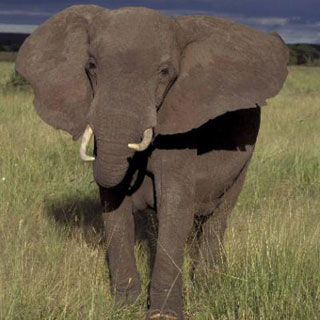
\includegraphics[width=0.8\linewidth]{elephant}
		\end{center}
		\blindtext[1]


\end{multicols}
% -----


%---
\section*{What a wonderful world}
This is such a wonderful document


\appendix

\section{Contact Information}
\subsection{Officers and Appointees}

\subsection{Note on Online Renewals}

\section{Membership Form}

%----
\end{document} 

